% Drawing 74/04-4 -- folder 74, batch 04, archive page 63 (PDF page 64).
% Transcription: un prisme vu en perspective, coupé en trois étages par des triangles horizontaux, les arêtes verticales reliant les étages.
% Kind: prism cut in three tiers. Method 2 (schematic redraw from the facsimile). Status: ok.
% Notes: A triangular prism in perspective, cut by two horizontal triangles into three tiers; the vertical edges join the tiers. The front edges are drawn as on the page; the structure (three stacked triangular prisms) is clear but it is left as a redraw because the middle triangles are internal membranes, not faces of a closed surface.
% Coordinates: 1 unit = 1 mm = 1/100 of the crop width (bbox in page fractions: [0.18, 0.12, 0.32, 0.27]).
% Redrawn by Claude (claude-opus-5-5), issue #73, 2026-11-07; not checked by a human; not compiled (no TeX in the session).
% Rights: reproduces part of the work -- behind RENDER_TRANSCRIPTS, never published by itself.
\documentclass[tikz,border=3pt]{standalone}
\usepackage{amsmath,amssymb}
\usetikzlibrary{patterns,arrows.meta}
\tikzset{pencil/.style={black!45}, struck/.style={black!35}, mark/.style={circle,draw,inner sep=1.3pt}, pt/.style={circle,fill,inner sep=0.9pt}, opt/.style={circle,draw,fill=white,inner sep=1.1pt}}
\begin{document}
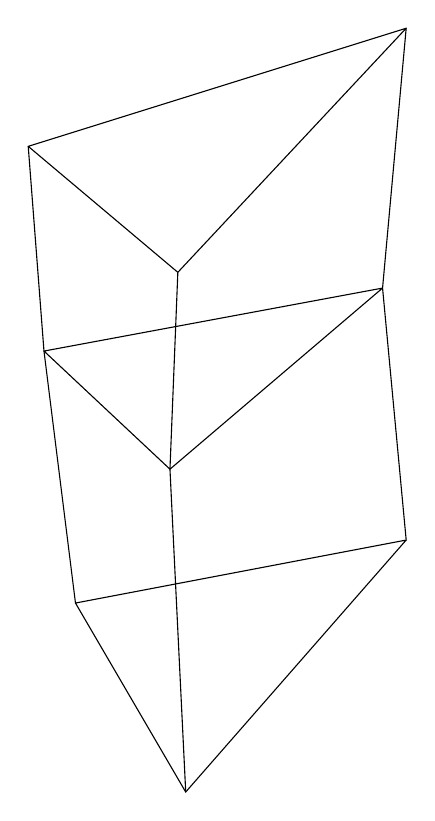
\begin{tikzpicture}[x=1mm,y=1mm,line cap=round,line join=round,font=\scriptsize]
\draw (30,-48) -- (78,-33) -- (49,-64) -- cycle;
\draw (32,-74) -- (75,-66) -- (48,-89) -- cycle;
\draw (36,-106) -- (78,-98) -- (50,-130) -- cycle;
\draw (30,-48) -- (32,-74) -- (36,-106);
\draw (78,-33) -- (75,-66) -- (78,-98);
\draw (49,-64) -- (48,-89) -- (50,-130);
\end{tikzpicture}
\end{document}
